\documentclass[border=2pt]{standalone}
\usepackage{amsmath, amsthm, amsfonts}
\usepackage{tikz-cd, kotex}
\usepackage{quiver}
\usepackage{Operators}
\usepackage{palette}
\usepackage{diagram-style}
\begin{document}

%%FIG counterexample_1 (Uniqueness_of_Submanifold-1.svg)
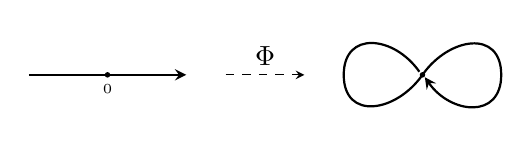
\begin{tikzpicture}
	\draw[thick, -{stealth}] (-5,0)--(-3,0);
	\fill (-4,0) circle[radius=1pt] node[below]{\tiny $0$};
	\draw[dashed, -{stealth}] (-2.5,0)--(-1.5,0) node[midway, above]{$\Phi$};
	\draw[thick] (0,0) to[out=55, in=90, looseness=1.5] (1,0);
	\draw[thick, -{stealth}] (1,0) to[out=-90, in=-55, looseness=1.5] (0.03,-0.03);
	\draw[thick] (-.04,.04) to[out=125, in=90, looseness=1.5] (-1,0);
	\draw[thick] (-1,0) to[out=-90, in=-125, looseness=1.5] (0,0);
	\fill (0,0) circle[radius=1pt];
\end{tikzpicture}

%%FIG counterexample_2 (Uniqueness_of_Submanifold-2.svg)
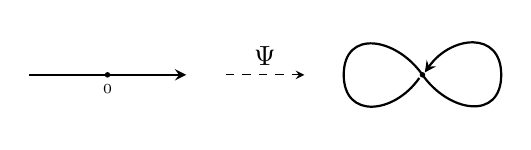
\begin{tikzpicture}
	\draw[thick, -{stealth}] (-5,0)--(-3,0);
	\fill (-4,0) circle[radius=1pt] node[below]{\tiny $0$};
	\draw[dashed, -{stealth}] (-2.5,0)--(-1.5,0) node[midway, above]{$\Psi$};
	\draw[thick, {stealth}-] (0.03,0.03) to[out=55, in=90, looseness=1.5] (1,0);
	\draw[thick] (1,0) to[out=-90, in=-55, looseness=1.5] (0,0);
	\draw[thick] (0,0) to[out=125, in=90, looseness=1.5] (-1,0);
	\draw[thick] (-1,0) to[out=-90, in=-125, looseness=1.5] (-0.04,-0.04);
	\fill (0,0) circle[radius=1pt];
\end{tikzpicture}

%%FIG counterexample_3 (Uniqueness_of_Submanifold-3.svg)
\begin{tikzpicture}
	\draw[thick, -{stealth}] (-5,0)--(-3,0);
	\draw[accent1, Parenthesis-Parenthesis, very thick] (-4.5,0)--(-3.5,0);
	\fill[accent1] (-4,0) circle[radius=1pt] node[below]{\tiny $0$};
	\draw[dashed, -{stealth}] (-2.5,0)--(-1.5,0) node[midway, above]{$\Phi$};
	\draw[thick] (0,0) to[out=55, in=90, looseness=1.5] (1,0);
	\draw[thick, -{stealth}] (1,0) to[out=-90, in=-55, looseness=1.5] (0.03,-0.03);
	\draw[thick] (-.04,.04) to[out=125, in=90, looseness=1.5] (-1,0);
	\draw[thick] (-1,0) to[out=-90, in=-125, looseness=1.5] (0,0);
	\fill (0,0) circle[radius=1pt];
	\begin{scope}
		\clip (0,0) circle[radius=10pt];
		\draw[accent1, thick] (0,0) to[out=55, in=90, looseness=1.5] (1,0);
		\draw[accent1, thick] (-1,0) to[out=-90, in=-125, looseness=1.5] (0,0);
		\fill[accent1] (0,0) circle[radius=1pt];
    \end{scope}
    \draw[double] (0,-1)--(0,-2);
	\draw[thick, -{stealth}] (-5,-3)--(-3,-3);
	\fill[accent1] (-4,-3) circle[radius=1pt] node[below]{\tiny $0$};
	\draw[dashed, {stealth}-] (-2.5,-3)--(-1.5,-3) node[midway, above]{$\bar{\Psi}^{-1}$};
	\draw[thick, {stealth}-] (0.03,-2.97) to[out=55, in=90, looseness=1.5] (1,-3);
	\draw[thick] (1,-3) to[out=-90, in=-55, looseness=1.5] (0,-3);
	\draw[thick] (0,-3) to[out=125, in=90, looseness=1.5] (-1,-3);
	\draw[thick] (-1,-3) to[out=-90, in=-125, looseness=1.5] (-0.04,-3.04);
	\fill (0,-3) circle[radius=1pt];
	\begin{scope}
		\clip (0,-3) circle[radius=10pt];
		\draw[accent1, thick, {stealth}-] (0.03,-2.97) to[out=55, in=90, looseness=1.5] (1,-3);
		\draw[accent1, thick] (-1,-3) to[out=-90, in=-125, looseness=1.5] (-0.04,-3.04);
		\fill[accent1] (0,-3) circle[radius=1pt];
    \end{scope}
    \draw[accent1, very thick, Parenthesis-{stealth}] (-3.5,-3)--(-3,-3);
    \draw[accent1, very thick, Parenthesis-] (-4.5,-3)--(-5,-3);
    \draw[dashed, -{stealth}] (-4,-1)--(-4,-2) node[midway, left]{$\bar{\Psi}^{-1}\circ\Phi$};
\end{tikzpicture}

%%FIG uniqueness (Uniqueness_of_Submanifold-4.svg)
\begin{tikzcd}
	{(A,\mathcal{T}',\mathcal{A}')} & M \\
	& {(A,\mathcal{T},\mathcal{A})}
	\arrow["{\iota'}", from=1-1, to=1-2]
	\arrow["\iota"', from=2-2, to=1-2]
	\arrow["{\operatorname{id}}"', dashed, from=1-1, to=2-2]
\end{tikzcd}

\end{document}
